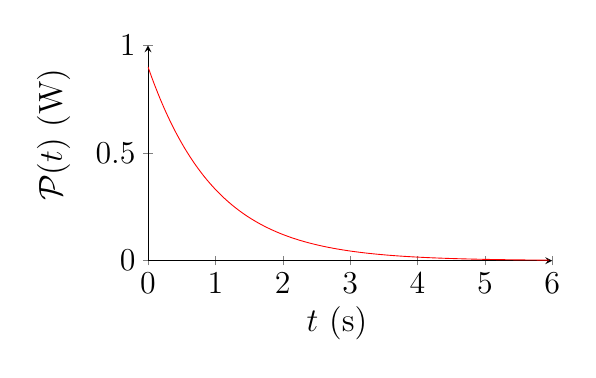
\begin{tikzpicture}[scale=0.8]
\shorthandoff{:!}
\begin{axis}[
	width=8cm, height=5cm,
	axis lines = left,
	xmin=0,xmax=6,
	ymin=0,ymax=1,
	xtick distance=1,
	ytick distance=0.5,
    xlabel = {},ylabel = {},
	tick label style={font=\Large},
]
%
\addplot [
    domain=0:5.95, 
    samples=200, 
    color=red,
]
{9/10*exp(-x)};

\end{axis}
\draw  (-1.5cm,2cm) node[rotate=90]{\large $\mathcal{P}(t)$ (\si{W})};
\draw  (3cm,-1.cm) node[]{\large $t$ (\si{s})};
\shorthandon{:!}
\end{tikzpicture}